\begin{question}
\noindent A UI/UX designer is scaling up an icon on a design grid so it can be used as a large app logo. The icon is triangle $L$, and it must be enlarged by scale factor $2$ using centre of enlargement $C$.

\begin{center}
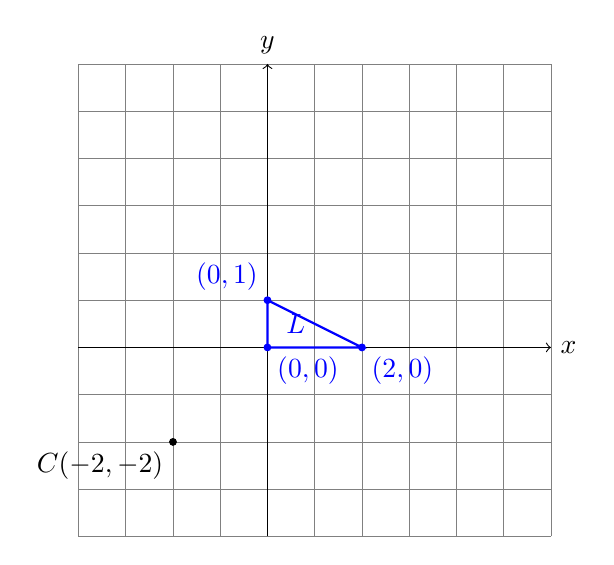
\begin{tikzpicture}[scale=0.6]
    \draw[step=1cm, gray, very thin] (-4,-4) grid (6,6);
    \draw[->] (-4,0) -- (6,0) node[right]{$x$};
    \draw[->] (0,-4) -- (0,6) node[above]{$y$};

    % Centre of enlargement C at (-2,-2)
    \filldraw[black] (-2,-2) circle (2pt) node[below left]{$C(-2,-2)$};

    % Triangle L vertices at (0,0), (2,0), (0,1)
    \draw[thick, blue] (0,0) -- (2,0) -- (0,1) -- cycle;
    \filldraw[blue] (0,0) circle (2pt) node[below right]{$(0,0)$};
    \filldraw[blue] (2,0) circle (2pt) node[below right]{$(2,0)$};
    \filldraw[blue] (0,1) circle (2pt) node[above left]{$(0,1)$};
    \node[blue] at (0.6,0.5) {$L$};
\end{tikzpicture}
\end{center}

\noindent On a grid like the one shown, enlarge triangle $L$ by scale factor $2$, using $C(-2,-2)$ as the centre of enlargement.

Write down the coordinates of the vertices of the enlarged triangle $L'$.

\vspace{5cm}
\answerplain{3}
\end{question}